% Shared preamble for the CIG-AMF formal-research papers.
% IEEEtran conference class; compiles on Overleaf without modification.
\documentclass[conference]{IEEEtran}
\IEEEoverridecommandlockouts

\usepackage{cite}
\usepackage{amsmath,amssymb,amsfonts}
\usepackage{amsthm}
\usepackage{algorithm}
\usepackage{algorithmic}
\usepackage{graphicx}
\usepackage{textcomp}
\usepackage{xcolor}
\usepackage{booktabs}
\usepackage{url}
\usepackage[hidelinks]{hyperref}

\def\BibTeX{{\rm B\kern-.05em{\sc i\kern-.025em b}\kern-.08em T\kern-.1667em\lower.7ex\hbox{E}\kern-.125emX}}

\newtheorem{theorem}{Theorem}
\newtheorem{lemma}[theorem]{Lemma}
\newtheorem{proposition}[theorem]{Proposition}
\newtheorem{corollary}[theorem]{Corollary}
\theoremstyle{definition}
\newtheorem{definition}[theorem]{Definition}
\newtheorem{remark}[theorem]{Remark}
\newtheorem{example}[theorem]{Example}

% A machine-checked statement carries its Lean declaration name.
\newcommand{\lean}[1]{\textsf{\footnotesize #1}}
\newcommand{\leanbox}[1]{%
  \par\vspace{2pt}\noindent
  {\footnotesize\textsf{Lean: #1}}\par\vspace{2pt}}

% Evidence classes, used consistently and never interchangeably.
\newcommand{\PROVED}{\textsc{proved}}
\newcommand{\CERT}{\textsc{certificate}}
\newcommand{\NUM}{\textsc{numerical}}
\graphicspath{{../_figures/}}


\begin{document}

\title{When the Extrema Move, the Scalar Proxy Fails\\
in Both Directions:\\
Solving the Group-Range Alternative Exactly}

\author{\IEEEauthorblockN{Vu Phan An Nguyen}
\IEEEauthorblockA{\textit{Rider University} \\
Lawrenceville, NJ, USA}}

\maketitle

\begin{abstract}
A design buys observations to certify the Top-$k$ of a set of relations ranked by
\emph{capacity}---the range $\max_{a}\theta_{ra}-\min_{a}\theta_{ra}$. Certifying means
excluding every alternative that would change the answer, so the design's value is the
energy of the cheapest such alternative. Allocators are routinely built on a scalar
pair-flip proxy $J_{\mathrm{scalar}}$, computed at the \emph{current} extrema with ordering
constraints dropped, because it is cheap. We show what that costs when the extrema can
move, and the answer is that it costs everything: we construct two explicit two-relation,
three-action families in exact arithmetic, one driving $J_{\mathrm{full}}/J_{\mathrm{scalar}}$
to $0$ and the other driving it to $+\infty$, so the proxy is a bound in neither direction
and no constant correction repairs it. We then solve the true problem. The alternative set
is a finite union of convex pair regions on the real range target, with the extrema chosen
from the alternative and never frozen at truth; a number lower-bounds the energy over the
whole set if and only if it does so on every region, so the oracle is a finite conjunction
of convex problems; the range constraints admit exact shrink and expand equivalences; the
inner quadratic programme has a closed form with a harmonic denominator; and the optimality
certificate is proved from primal feasibility, dual non-negativity, stationarity and
complementary slackness using only symmetry and positive \emph{semi}definiteness, so a
singular information matrix costs no extra hypothesis and no pseudoinverse. Everything is
machine-checked in Lean~4 with no \texttt{sorry}. On a confirmatory panel of $1000$ paired
instances, $\mathrm{C\_lucb}$ certifies $797$ worlds at median $20{,}996$ queries against
$605$ at $74{,}252$ for uniform.
\end{abstract}

\begin{IEEEkeywords}
best-arm identification, experimental design, convex optimisation, KKT conditions,
counterexamples, formal verification, interactive theorem proving
\end{IEEEkeywords}

\section{Introduction}

A design buys observations in order to \emph{certify} an answer, not merely to estimate a
parameter. The answer here is the Top-$k$ of a set of relations ranked by their capacity,
\begin{equation}
C_{r}(\theta)\;=\;\max_{a}\theta_{ra}\;-\;\min_{a}\theta_{ra},
\label{eq:capacity}
\end{equation}
and certifying means excluding every alternative parameter that would change the answer.
The design's value is therefore the energy of the cheapest such alternative---an infimum
over a set, not a variance at a point.

\subsection{Three quantities that must be kept apart}

Three related numbers appear in this problem and are easily conflated.
$J_{\mathrm{scalar}}$ is the pair-flip value computed at the \emph{current} extrema with the
ordering constraints dropped. $J_{\mathrm{old}}$ is the quadratic programme inside the
current-extrema region. $J_{\mathrm{full}}$ is the infimum over the whole alternative set,
with the extrema free in either relation. By inclusion of feasible sets,
\begin{equation}
J_{\mathrm{scalar}}\;\leq\;J_{\mathrm{old}},
\qquad
J_{\mathrm{full}}\;\leq\;J_{\mathrm{old}},
\label{eq:order}
\end{equation}
and---this is the point of the paper---there is \emph{no} general order between
$J_{\mathrm{scalar}}$ and $J_{\mathrm{full}}$.

Allocators are routinely built on $J_{\mathrm{scalar}}$ because it is cheap: it is a
one-dimensional computation at a fixed pair of cells. This work asks what that costs when
the extrema can move, and Section~\ref{sec:families} answers it with two explicit families.

\subsection{Why a range target is not a mean target}

The difficulty is specific to ranking by a range, and it is worth isolating before the
formalism.

When relations are ranked by a mean, the comparison $\mu_{j}\ge\mu_{i}$ is a single linear
inequality, so the relevant alternative set is a half-space---convex, with one facet, and
with a closed-form nearest point under any quadratic energy. The inner problem has a
harmonic denominator over two precisions and there is nothing further to decide.

When relations are ranked by a range, the comparison
$C_{j}(\lambda)\ge C_{i}(\lambda)$ hides four extremal choices, and which cells attain them
depends on $\lambda$. The set
$\{\lambda:C_{j}(\lambda)\ge C_{i}(\lambda)\}$ is not convex: it is a union of polyhedra,
one per choice of attaining pair, and the minimiser may sit in a piece whose attaining cells
differ from the truth's. Any procedure that fixes the attaining cells in advance is
therefore solving a restriction of the problem, and a restriction can have a strictly larger
value.

That last sentence is the entire mechanism behind family~1. Family~2 shows the reverse
failure, which arises from the other approximation---dropping the ordering constraints that
define a piece---and the two together are what make Corollary~\ref{cor:noconstant} possible.

\subsection{Contributions}

\begin{enumerate}
\item[C1.] \textbf{The scalar proxy is wrong in both directions, by no constant.} Two
explicit two-relation, three-action families. In the first $J_{\mathrm{full}}/J_{\mathrm{scalar}}$
is driven to $0$; in the second to $+\infty$ (Theorems~\ref{thm:family1},
\ref{thm:family2}). Both are exact-arithmetic constructions with explicit feasible
alternatives and elementary lower bounds---no optimiser, no sampled world, no seed---so no
constant correction can repair the proxy.

\item[C2.] \textbf{The true alternative set is a finite union of convex pair regions.} A
finite max/min set identity on the real \emph{range} target, not a Top-1 surrogate, with the
extrema chosen from the alternative and never frozen at truth (Theorem~\ref{thm:union});
each region is convex with no definiteness assumption on any observation matrix
(Proposition~\ref{prop:convex}).

\item[C3.] \textbf{The energy oracle becomes a finite check.} A number lower-bounds the
energy over the whole alternative set if and only if it does so on every pair region
(Theorem~\ref{thm:oracle}), so certifying is a finite conjunction of convex problems and no
infimum over an infinite-dimensional set is ever taken.

\item[C4.] \textbf{Shrink and expand, as equivalences.} Range $\le z$ iff all cells lie in a
common interval of length $z$, minimised coordinate-wise by the clamp; range $\ge z$ iff
some \emph{ordered} pair is separated by at least $z$, so no third cell has to move
(Theorems~\ref{thm:shrink}, \ref{thm:expand}). Both directions are equivalences, so nothing
is relaxed.

\item[C5.] \textbf{An optimality certificate that needs no matrix inverse.} The textbook
dual requires $M$ invertible. We prove optimality from primal feasibility, dual
non-negativity, stationarity and complementary slackness using only symmetry and positive
\emph{semi}definiteness (Theorem~\ref{thm:kkt}).

\item[C6.] \textbf{The setup-cost law, with infeasibility reported as infeasibility.} An
infeasible configuration has \emph{no} value and is never clamped to a small positive one;
the crossing budget between two supports is derived, and when the two values are only
bracketed we prove both orders remain consistent, so the honest output is
\textsc{undecided} (Theorems~\ref{thm:crossing}, \ref{thm:undecided}).
\end{enumerate}

\subsection{Roadmap}

Section~\ref{sec:setting} fixes notation and Section~\ref{sec:related} the novelty boundary.
Sections~\ref{sec:union}--\ref{sec:kkt} solve the true problem: the union identity, the
finite oracle, the shrink/expand equivalences, the inner closed form and the inverse-free
certificate. Section~\ref{sec:families} gives the two counterexample families,
Section~\ref{sec:setup} the setup-cost law, Section~\ref{sec:results} the panel,
Section~\ref{sec:verification} the formal development and Section~\ref{sec:discussion} the
scope---which is unusually long here, because the full oracle equality is \emph{not}
assembled and saying so precisely matters.

\section{Setting and notation}
\label{sec:setting}

\begin{table}[htbp]
\caption{Notation.}
\label{tab:notation}
\centering
\footnotesize
\begin{tabular}{@{}ll@{}}
\toprule
Symbol & Meaning \\
\midrule
$r,i,j$ & relation indices; $i\in T$, $j\notin T$ \\
$a,b,u,v$ & action indices \\
$\theta_{ra}$ & true parameter at relation $r$, action $a$ \\
$\lambda$ & an alternative parameter \\
$C_{r}$ & capacity, \eqref{eq:capacity} \\
$T$ & the claimed Top-$k$ set \\
$\alpha_{ra}$ & precision purchased at cell $(r,a)$ \\
$x,w$ & design (allocation) vectors \\
$M(x)$ & information matrix at design $x$ \\
$\mathcal{P}_{ijab}$ & pair region, \eqref{eq:polyhedron} \\
$J_{\mu}(x)$ & full energy oracle, \eqref{eq:J} \\
$S_{i}(z)$ & shrink cost of relation $i$ to range $z$ \\
$E_{j}(z)$ & expand cost of relation $j$ to range $z$ \\
$[\,\cdot\,]_{+}$ & positive part \\
$\eta$ & family parameter, $0<\eta\le1$ \\
$\Gamma_{1},\Gamma_{2}$ & per-support rates \\
$B_{*}$ & crossing budget, \eqref{eq:crossing} \\
\bottomrule
\end{tabular}
\end{table}

The design buys precision $\alpha_{ra}$ at each cell and the energy of an alternative
$\lambda$ is the quadratic form $\tfrac12(\lambda-\mu)^{\top}M(x)(\lambda-\mu)$. An
alternative is \emph{relevant} if it would change the Top-$k$ answer, i.e.\ if some
$j\notin T$ overtakes some $i\in T$ in capacity.

\subsection{What the scalar proxy is, exactly}
\label{sec:proxydef}

Since the paper's first claim is that a particular approximation fails, the approximation
must be pinned down. Given the truth $\mu$, a claimed top relation $i$ and a challenger $j$,
let $a^{\circ},b^{\circ}$ be the cells attaining $i$'s current max and min, and
$c^{\circ},d^{\circ}$ those attaining $j$'s. The scalar proxy is the value of the inner
problem \eqref{eq:innerqp} at those four cells with the ordering constraints dropped:
\begin{equation}
J_{\mathrm{scalar}}
\;=\;
\frac{\bigl(C_{i}(\mu)-C_{j}(\mu)\bigr)^{2}}
     {2\Bigl(\frac{1}{\alpha_{ia^{\circ}}}+\frac{1}{\alpha_{ib^{\circ}}}
            +\frac{1}{\alpha_{jc^{\circ}}}+\frac{1}{\alpha_{jd^{\circ}}}\Bigr)} .
\label{eq:scalar}
\end{equation}

Two approximations are folded into \eqref{eq:scalar}, and they fail independently. The
first is that the extrema stay where they are: the four cells are read off $\mu$ and never
revisited, so an alternative that changes which cell is extremal is invisible. The second
is that the ordering constraints defining $\mathcal{P}_{ijab}$ are dropped, so an
alternative that would have to satisfy them is charged too little. Family~1 of
Section~\ref{sec:families} exploits the first, family~2 the second, and each drives the
error in a different direction.

It is worth being explicit that \eqref{eq:scalar} is not a strawman. It is the natural
transport of the fixed-confidence inner problem to this setting, it is cheap---four lookups
and an arithmetic expression---and it agrees with $J_{\mathrm{full}}$ whenever the extrema
happen not to move. The question is whether that agreement can be relied on, and
Corollary~\ref{cor:noconstant} says it cannot, even up to a constant.

\section{Related work and the novelty boundary}
\label{sec:related}

\subsection{Best-arm identification with unknown variances}

Jourdan, Degenne and Kaufmann \cite{jourdan2023} and Garivier and Kaufmann
\cite{garivier2016} develop the fixed-confidence best-arm identification framework in which
the stopping rule is a generalised likelihood-ratio statistic and the sampling rule tracks
the optimal-allocation weights. The alternative set in that literature is
$\{\lambda:\text{some arm }j\text{ beats arm }i\}$ with the comparison on the arm
\emph{means}, and the resulting inner problem is a one-dimensional convex programme with a
closed form---the familiar harmonic denominator.

The present problem differs in the object being compared. Capacity \eqref{eq:capacity} is a
range, so the comparison $C_{j}(\lambda)\ge C_{i}(\lambda)$ involves a maximum and a minimum
over actions in \emph{each} relation, and the extrema attaining them depend on $\lambda$.
The alternative set is therefore not a half-space but a union of polyhedra, and the
literature's inner problem is recovered only on one piece of that union with the extrema
frozen. Section~\ref{sec:families} shows the error made by freezing them.

\subsection{Convex optimisation and KKT}

The certificate of Section~\ref{sec:kkt} is a standard sufficiency argument for a convex
quadratic programme \cite{boyd2004}. What is not standard is that it is carried through
without assuming $M$ invertible: the textbook derivation of the dual eliminates the primal
variable using $M^{-1}$, and at a sparse allocation---which is exactly where a design
algorithm operates---$M$ is singular. Theorem~\ref{thm:kkt} is stated so that positive
semidefiniteness suffices.

\subsection{Summary of the boundary}

Claimed as new: the two-directional failure of the scalar proxy with explicit families (C1);
the union identity on the range target with free extrema (C2); the finite-check oracle (C3);
the shrink/expand equivalences (C4); the inverse-free certificate (C5); and the setup-cost
law with honest infeasibility (C6). The fixed-confidence framework, the harmonic
denominator in its own setting, and convex duality are cited.

\section{The alternative set}
\label{sec:union}

\subsection{The finite max/min set identity}

\begin{theorem}[Union identity]
\label{thm:union}
For relations $i,j$ and any alternative $\lambda$,
\begin{multline}
C_{j}(\lambda)\geq C_{i}(\lambda)
\;\;\Longleftrightarrow\;\;
\exists\,a,b\;\;\forall\,u,v:\\
\lambda_{ja}-\lambda_{jb}\;\geq\;\lambda_{iu}-\lambda_{iv}.
\label{eq:union}
\end{multline}
\end{theorem}

\begin{proof}
($\Rightarrow$) Choose $a$ attaining $\max_{a}\lambda_{ja}$ and $b$ attaining
$\min_{b}\lambda_{jb}$, so $\lambda_{ja}-\lambda_{jb}=C_{j}(\lambda)$. For any $u,v$ we have
$\lambda_{iu}-\lambda_{iv}\le C_{i}(\lambda)\le C_{j}(\lambda)$, which is the right-hand
side.

($\Leftarrow$) Given such $a,b$, the range of $j$ is at least
$\lambda_{ja}-\lambda_{jb}$, which by hypothesis dominates every pair difference in $i$.
Taking the maximum over $i$'s pairs, the right-hand side dominates $C_{i}(\lambda)$, so
$C_{j}(\lambda)\ge C_{i}(\lambda)$.
\end{proof}

\leanbox{\lean{range\_ge\_iff\_exists\_pair} in
\lean{LeanFunctionalRangeAlternativeUnionV1}}

This is the model bridge and the step that makes everything else possible. It converts a
statement about extrema---objects that move with $\lambda$---into a statement about a
\emph{fixed} pair $(a,b)$, at the cost of an existential over finitely many pairs. Crucially
the extrema are chosen from the alternative, never frozen at the truth; freezing them is
exactly the error Section~\ref{sec:families} quantifies.

\subsection{A union of polyhedra}

\begin{definition}[Pair region]
\begin{equation}
\mathcal{P}_{ijab}=\bigl\{\lambda:\;
\lambda_{iu}-\lambda_{iv}-\lambda_{ja}+\lambda_{jb}\leq 0
\;\;\forall u,v\bigr\}.
\label{eq:polyhedron}
\end{equation}
\end{definition}

\begin{proposition}[Convexity, unconditionally]
\label{prop:convex}
Each $\mathcal{P}_{ijab}$ is convex, with no assumption on $M$.
\end{proposition}

\begin{proof}
Each defining constraint in \eqref{eq:polyhedron} is linear in $\lambda$, so the region is
an intersection of half-spaces.
\end{proof}

\leanbox{\lean{alternative\_union\_polyhedra}, \lean{pairRegion\_convex} in
\lean{LeanFunctionalRangeAlternativeUnionV1}}

By Theorem~\ref{thm:union} the relevant alternative set is the finite union
$\bigcup_{i,j,a,b}\mathcal{P}_{ijab}$, and the oracle is
\begin{equation}
J_{\mu}(x)\;=\;\min_{i\in T,\,j\notin T,\,a,b}\;
\inf_{\lambda\in\mathcal{P}_{ijab}}\;
\tfrac{1}{2}(\lambda-\mu)^{\top}M(x)(\lambda-\mu).
\label{eq:J}
\end{equation}

\section{The oracle is a finite check}
\label{sec:oracle}

\begin{theorem}[Finite check]
\label{thm:oracle}
A number $c$ lower-bounds the energy over the whole alternative set if and only if it
lower-bounds it on every pair region.
\end{theorem}

\begin{proof}
($\Leftarrow$) Any $\lambda$ in the union lies in some region by
Theorem~\ref{thm:union}, so its energy is at least $c$. ($\Rightarrow$) Each region is a
subset of the union.
\end{proof}

\leanbox{\lean{energy\_lower\_bound\_iff}, \lean{energy\_ge\_of\_pairwise} in
\lean{LeanFunctionalRangeEnergyOracleV1}}

The index set in \eqref{eq:J} is finite, so certifying reduces to a finite conjunction of
convex problems. No infimum over an infinite-dimensional set is ever taken, which is the
computational content of C3.

\begin{remark}[Directions are never conflated]
A lower bound valid for \emph{every} region, and then their minimum, lower-bounds $J$. A
single feasible alternative only \emph{upper}-bounds it. The distinction is maintained
throughout the development and in the formal statements: \lean{energy\_ge\_of\_pairwise}
concludes a lower bound from a universally quantified hypothesis, and nothing in the
development derives a lower bound from an exhibited point.
\end{remark}

\section{Shrink and expand}
\label{sec:shrink}

Certifying against a pair region reduces to two one-sided problems: shrinking the incumbent
$i$'s range below a level $z$ and expanding the challenger $j$'s above it. Both are
equivalences.

\begin{theorem}[Shrink]
\label{thm:shrink}
$\mathrm{range}(\theta_{i})\le z$ if and only if all cells of $i$ lie in a common interval
of length $z$, and the cheapest such placement is coordinate-wise the clamp:
\begin{equation}
S_{i}(z)=\min_{\ell}\,\frac{1}{2}\sum_{a}\alpha_{ia}\;
\mathrm{dist}\bigl(\theta_{ia},\,[\ell,\ell+z]\bigr)^{2}.
\label{eq:shrink}
\end{equation}
\end{theorem}

\begin{proof}
The equivalence is immediate from the definition of range. For the cost, fix $\ell$; for
each cell independently the closest point of $[\ell,\ell+z]$ to $\theta_{ia}$ is the clamp,
proved by cases on whether $\theta_{ia}$ lies below, inside or above the interval. The
per-cell costs then sum because the objective is separable given $\ell$.
\end{proof}

\leanbox{\lean{range\_le\_iff\_exists\_interval}, \lean{clamp\_dist\_le},
\lean{shrink\_lower} in \lean{LeanFunctionalShrinkExpandV1}}

\begin{theorem}[Expand]
\label{thm:expand}
$\mathrm{range}(\theta_{j})\ge z$ if and only if some \emph{ordered} pair is separated by at
least $z$, and
\begin{equation}
E_{j}(z)=\min_{a\neq b}\;
\frac{\bigl[\,z-(\theta_{ja}-\theta_{jb})\,\bigr]_{+}^{2}}
     {2\bigl(\frac{1}{\alpha_{ja}}+\frac{1}{\alpha_{jb}}\bigr)}.
\label{eq:expand}
\end{equation}
\end{theorem}

\begin{proof}
The equivalence is again immediate. For the cost, the problem is to minimise a separable
quadratic subject to \emph{one} linear constraint $\lambda_{ja}-\lambda_{jb}\ge z$; the
minimiser is exhibited explicitly and the value computed by substitution, so the expression
is exact rather than bounded.
\end{proof}

\leanbox{\lean{range\_ge\_iff\_exists\_pair\_ge}, \lean{expand\_lower} in
\lean{LeanFunctionalShrinkExpandV1}}

The word \emph{ordered} in Theorem~\ref{thm:expand} is load-bearing. Requiring an ordered
pair means only two cells move; an unordered formulation would force a third cell to
accommodate the separation and would overstate the cost.

\section{The inner problem in closed form}
\label{sec:innerqp}

\begin{theorem}[Inner quadratic programme]
\label{thm:innerqp}
For weights $w_{i}>0$ and $g\in\mathbb{R}$,
\begin{equation}
\min\;\frac{1}{2}\sum_{i=1}^{4}w_{i}x_{i}^{2}
\;\;\text{s.t.}\;\;x_{1}-x_{2}-x_{3}+x_{4}\geq g
\;=\;
\frac{g^{2}}{2\sum_{i=1}^{4}\frac{1}{w_{i}}} .
\label{eq:innerqp}
\end{equation}
\end{theorem}

\begin{proof}
Completing the square against the explicit minimiser
$x_{i}^{*}=\pm g/(w_{i}\sum_{k}w_{k}^{-1})$ with signs matching the constraint's
coefficients. No optimiser and no multiplier theorem is invoked; the identity is verified by
substitution and the inequality by the square-completion residual.
\end{proof}

\leanbox{\lean{inner\_qp\_lower}, \lean{inner\_qp\_attained}, \lean{harm\_pos} in
\lean{LeanFunctionalRangeEnergyOracleV1}}

The harmonic denominator is the same shape that appears in the fixed-confidence literature,
but it is \emph{derived here for the range target} rather than transported from a Top-1
surrogate. The difference is the four terms: a range comparison moves two cells in each of
two relations, so the harmonic sum runs over four precisions rather than two.

\section{The certificate, without an inverse}
\label{sec:kkt}

\begin{theorem}[KKT sufficiency under semidefiniteness]
\label{thm:kkt}
Let $M$ be symmetric positive semidefinite, $A$ the constraint matrix of a pair region, and
suppose $\lambda^{*}$ and $y$ satisfy
\begin{equation}
M(\lambda^{*}-\mu)+A^{\top}y=0,\quad
y\geq 0,\quad
A\lambda^{*}\leq 0,\quad
y^{\top}A\lambda^{*}=0 .
\label{eq:kkt}
\end{equation}
Then $\lambda^{*}$ minimises the energy over the region.
\end{theorem}

\begin{proof}
Let $\lambda$ be any feasible competitor and write $d=\lambda-\lambda^{*}$. Expanding the
quadratic at $\lambda$,
\begin{align}
&\tfrac12(\lambda-\mu)^{\top}M(\lambda-\mu)
 -\tfrac12(\lambda^{*}-\mu)^{\top}M(\lambda^{*}-\mu) \notag\\
&\qquad=\;d^{\top}M(\lambda^{*}-\mu)\;+\;\tfrac12 d^{\top}Md .
\end{align}
By stationarity $M(\lambda^{*}-\mu)=-A^{\top}y$, so the cross term is
$-d^{\top}A^{\top}y=-y^{\top}A\lambda+y^{\top}A\lambda^{*}=-y^{\top}A\lambda$, using
complementary slackness. Feasibility of $\lambda$ gives $A\lambda\le0$ and $y\ge0$, so
$-y^{\top}A\lambda\ge0$. The remaining term $\tfrac12 d^{\top}Md$ is non-negative by
positive semidefiniteness. Hence the difference is non-negative.
\end{proof}

\leanbox{\lean{kkt\_certificate}, \lean{certificate\_gives\_lower\_bound} in
\lean{LeanFunctionalRangeDesignCertificateV1}}

No inverse appears anywhere in the proof. This matters for practice as much as for rigour:
information matrices at sparse allocations are routinely singular, and a certificate that
survives singularity without a pseudoinverse is what makes the oracle usable at the boundary
of the design simplex---which is where an allocator that has concentrated its budget
actually sits.

\section{The oracle as a procedure}
\label{sec:procedure}

Sections~\ref{sec:union}--\ref{sec:kkt} assemble into a procedure. Stating it makes the
computational claim of C3 concrete and shows where each theorem is used.

\begin{enumerate}
\item \textbf{Enumerate the pairs.} For each $i\in T$, $j\notin T$ and each ordered pair of
actions $(a,b)$ of relation $j$, form the region $\mathcal{P}_{ijab}$ of
\eqref{eq:polyhedron}. By Theorem~\ref{thm:union} these cover the relevant alternative set
exactly---no alternative is missed and none is counted that would not change the answer.

\item \textbf{Solve each region.} Each is a convex quadratic programme by
Proposition~\ref{prop:convex}, and by Theorems~\ref{thm:shrink} and \ref{thm:expand} its
value decomposes as $\inf_{z\ge0}[S_{i}(z)+E_{j}(z)]$ over a scalar $z$: shrink the
incumbent below $z$, expand the challenger above it. Both one-sided costs are closed forms.

\item \textbf{Read the inner value.} Where a single pair of cells moves in each relation,
Theorem~\ref{thm:innerqp} gives the value directly with the four-term harmonic denominator,
so no numerical solve is needed on that piece.

\item \textbf{Certify.} A candidate minimiser with multipliers satisfying \eqref{eq:kkt} is
optimal by Theorem~\ref{thm:kkt}, and the certificate holds even when $M$ is singular---
which it is whenever the allocation is sparse.

\item \textbf{Take the minimum.} By Theorem~\ref{thm:oracle} the minimum over the finite
index set is the oracle value, and a lower bound valid on every region is a lower bound on
the whole set.
\end{enumerate}

\subsection{Cost}

The index set has size $|T|\cdot|T^{c}|\cdot|A|(|A|-1)$, which is polynomial in the problem
size and independent of any discretisation. Each piece is either a closed form (step~3) or a
one-dimensional minimisation over $z$ (step~2) whose integrand is a sum of two explicit
convex functions. Nothing in the procedure requires a general-purpose convex solver, and
nothing requires inverting $M$.

The contrast with \eqref{eq:scalar} is therefore not that the exact oracle is intractable
and the proxy is cheap; it is that the exact oracle is a finite enumeration of closed forms
and the proxy is one of them evaluated at the wrong index.

\section{The two families}
\label{sec:families}

Both families have two relations and three actions, with Top-1 claimed for relation $i$ and
a parameter $0<\eta\le1$.

\subsection{Family 1: the proxy overstates}

\begin{theorem}[$J_{\mathrm{full}}/J_{\mathrm{scalar}}\to0$]
\label{thm:family1}
Take
\begin{align}
\theta_{i}=(0,1,\tfrac12),\;\alpha_{i}=(1,1,1);\\
\theta_{j}=(0,\tfrac12,\tfrac14),\;\alpha_{j}=(1,1,\eta).
\end{align}
Then $J_{\mathrm{scalar}}=\tfrac{1}{32}$ while
\begin{equation}
0\;\leq\;\frac{J_{\mathrm{full}}}{J_{\mathrm{scalar}}}\;\leq\;9\eta
\;\xrightarrow[\eta\to0]{}\;0 .
\label{eq:family1}
\end{equation}
\end{theorem}

\begin{proof}
Raising \emph{only} the third cell of $j$ from $\tfrac14$ to $1$ equalises the two
capacities: $C_{j}$ becomes $1-0=1=C_{i}$. The energy of that move is
$\tfrac12\eta(1-\tfrac14)^{2}=\tfrac{9\eta}{32}$, so
$J_{\mathrm{full}}\le\tfrac{9\eta}{32}$. The scalar proxy, computed at the current extrema
of $j$ (cells $2$ and $1$, both at precision $1$) with ordering dropped, reports
$\tfrac{1}{32}$. Dividing gives \eqref{eq:family1}.
\end{proof}

\leanbox{\lean{scalar\_not\_upper\_to\_any\_constant} in
\lean{LeanFunctionalScalarProxyFailsV1}}

The mechanism is that the cheap way to raise $j$'s capacity is through a cell that is
\emph{not} currently an extremum, and the proxy cannot see it because it has frozen the
extrema at their current positions. As $\eta\to0$ that cell becomes arbitrarily cheap and
the true value collapses while the proxy does not move at all.

\subsection{Family 2: the proxy understates}

\begin{theorem}[$J_{\mathrm{full}}/J_{\mathrm{scalar}}\to+\infty$]
\label{thm:family2}
Take
\begin{align}
\theta_{i}=(0,1,\tfrac34),\;\alpha_{i}=(1,\eta,1);\\
\theta_{j}=(0,\tfrac12,\tfrac14),\;\alpha_{j}=(1,1,1).
\end{align}
Then $J_{\mathrm{full}}\ge\tfrac{1}{128}$ while
\begin{equation}
\frac{J_{\mathrm{full}}}{J_{\mathrm{scalar}}}
\;\geq\;\frac{1+3\eta}{16\eta}
\;\xrightarrow[\eta\to0]{}\;+\infty .
\label{eq:family2}
\end{equation}
\end{theorem}

\begin{proof}
Let $\lambda$ be \emph{any} capacity-inverting alternative and pick $z$ strictly between the
two new capacities. Shrinking $i$ below $z$ costs at least
$[\tfrac34-z]_{+}^{2}/4$ by Theorem~\ref{thm:shrink}, since the third cell of $i$ has
precision $1$ and must come down to $z$; opening $j$ above $z$ costs at least
$[z-\tfrac12]_{+}^{2}/4$ by Theorem~\ref{thm:expand}. The two positive parts always sum to
at least $\tfrac14$: by cases on $z$, if $z\le\tfrac12$ the first term is at least
$(\tfrac14)^{2}$, if $z\ge\tfrac34$ the second is at least $(\tfrac14)^{2}$, and in between
the two parts sum to exactly $\tfrac14$. Hence
$J_{\mathrm{full}}\ge\tfrac{1}{4}\cdot\tfrac{1}{32}=\tfrac{1}{128}$. Meanwhile the scalar
proxy, seeing the cheap cell of $i$ at precision $\eta$, reports
$\eta/(8(1+3\eta))$, and dividing gives \eqref{eq:family2}.
\end{proof}

\leanbox{\lean{scalar\_not\_lower\_to\_any\_constant}, \lean{positive\_parts\_sum},
\lean{family2\_full\_ge} in \lean{LeanFunctionalScalarProxyFailsV1}}

Here the mechanism is the reverse. The proxy sees a cheap route---move $i$'s second cell,
which has precision $\eta$---and concludes the alternative is nearly free. But moving that
cell alone does not inverting the capacities, because $i$'s range is set by its first and
third cells; the alternative must additionally pay on cells the proxy never examines, and
the positive-parts bound shows that payment cannot be avoided.

\subsection{The two families side by side}

\begin{table}[htbp]
\caption{The two families in full. Both have two relations and three actions and the same
true capacities $C_{i}=1$, $C_{j}=\tfrac12$, hence the same gap $g=\tfrac12$. They differ
only in where the small precision $\eta$ sits, and that placement determines the direction
in which the proxy errs.}
\label{tab:familydata}
\centering
\footnotesize
\setlength{\tabcolsep}{4pt}
\begin{tabular}{@{}lll@{}}
\toprule
 & Family 1 & Family 2 \\
\midrule
$\theta_{i}$ & $(0,1,\tfrac12)$ & $(0,1,\tfrac34)$ \\
$\alpha_{i}$ & $(1,1,1)$ & $(1,\eta,1)$ \\
$\theta_{j}$ & $(0,\tfrac12,\tfrac14)$ & $(0,\tfrac12,\tfrac14)$ \\
$\alpha_{j}$ & $(1,1,\eta)$ & $(1,1,1)$ \\
\midrule
harmonic sum & $4$ & $3+\tfrac1\eta$ \\
$J_{\mathrm{scalar}}$ & $\tfrac{1}{32}$ & $\dfrac{\eta}{8(1+3\eta)}$ \\
$J_{\mathrm{full}}$ & $\le\tfrac{9\eta}{32}$ & $\ge\tfrac{1}{128}$ \\
ratio & $\le 9\eta\to0$ & $\ge\dfrac{1+3\eta}{16\eta}\to\infty$ \\
\midrule
cheap cell & $j$'s third & $i$'s second \\
is it extremal? & no & yes \\
which approximation fails & frozen extrema & dropped ordering \\
\bottomrule
\end{tabular}
\end{table}

Table~\ref{tab:familydata} makes the symmetry visible. The two instances have the same
capacities, the same gap and the same shape; the only difference is which cell carries the
small precision $\eta$ and whether that cell is currently extremal.

In family~1 the cheap cell is \emph{not} extremal, so \eqref{eq:scalar} never looks at it
and computes a harmonic sum of $4$ regardless of $\eta$. The true cheapest alternative goes
straight through that cell, so $J_{\mathrm{full}}$ scales with $\eta$ while
$J_{\mathrm{scalar}}$ stays at $\tfrac{1}{32}$: the proxy \emph{overstates} without bound.

In family~2 the cheap cell \emph{is} extremal, so \eqref{eq:scalar} does look at it and its
harmonic sum blows up as $\eta\to0$, driving $J_{\mathrm{scalar}}$ to zero. But moving that
cell alone does not invert the capacities---$i$'s range is pinned by its first and third
cells---and the positive-parts bound shows every genuine alternative must pay at least
$\tfrac{1}{128}$ elsewhere. The proxy \emph{understates} without bound.

\subsection{The positive-parts inequality}

The lower bound in Theorem~\ref{thm:family2} rests on one elementary inequality, stated
separately because it is what makes the bound uniform over alternatives rather than
instance-by-instance.

\begin{lemma}[Positive parts]
\label{lem:posparts}
For every $z\in\mathbb{R}$,
\begin{equation}
\bigl[\tfrac34-z\bigr]_{+}\;+\;\bigl[z-\tfrac12\bigr]_{+}\;\geq\;\tfrac14 .
\end{equation}
\end{lemma}

\begin{proof}
Three cases. If $z\le\tfrac12$ the first part is $\tfrac34-z\ge\tfrac14$. If $z\ge\tfrac34$
the second is $z-\tfrac12\ge\tfrac14$. If $\tfrac12<z<\tfrac34$ both parts are positive and
sum to exactly $\tfrac34-\tfrac12=\tfrac14$.
\end{proof}

\leanbox{\lean{positive\_parts\_sum} in \lean{LeanFunctionalScalarProxyFailsV1}}

The lemma is what closes the quantifier in Theorem~\ref{thm:family2}. Without it one could
only say that \emph{some} alternatives are expensive; with it, \emph{every} capacity-
inverting alternative is, whatever $z$ it chooses, and the bound $\tfrac{1}{128}$ is a
property of the instance rather than of a particular competitor.

\subsection{Why this settles the question}

\begin{corollary}[No constant repairs the proxy]
\label{cor:noconstant}
There is no constant $c$ with $J_{\mathrm{full}}\le c\,J_{\mathrm{scalar}}$ for all
instances, and none with $J_{\mathrm{full}}\ge c\,J_{\mathrm{scalar}}$.
\end{corollary}

\begin{proof}
Family 2 refutes the first for every $c$, taking $\eta$ small enough that
$(1+3\eta)/(16\eta)>c$. Family 1 refutes the second, taking $\eta<c^{-1}\cdot$ the relevant
constant in \eqref{eq:family1}.
\end{proof}

\begin{figure}[htbp]
\centering
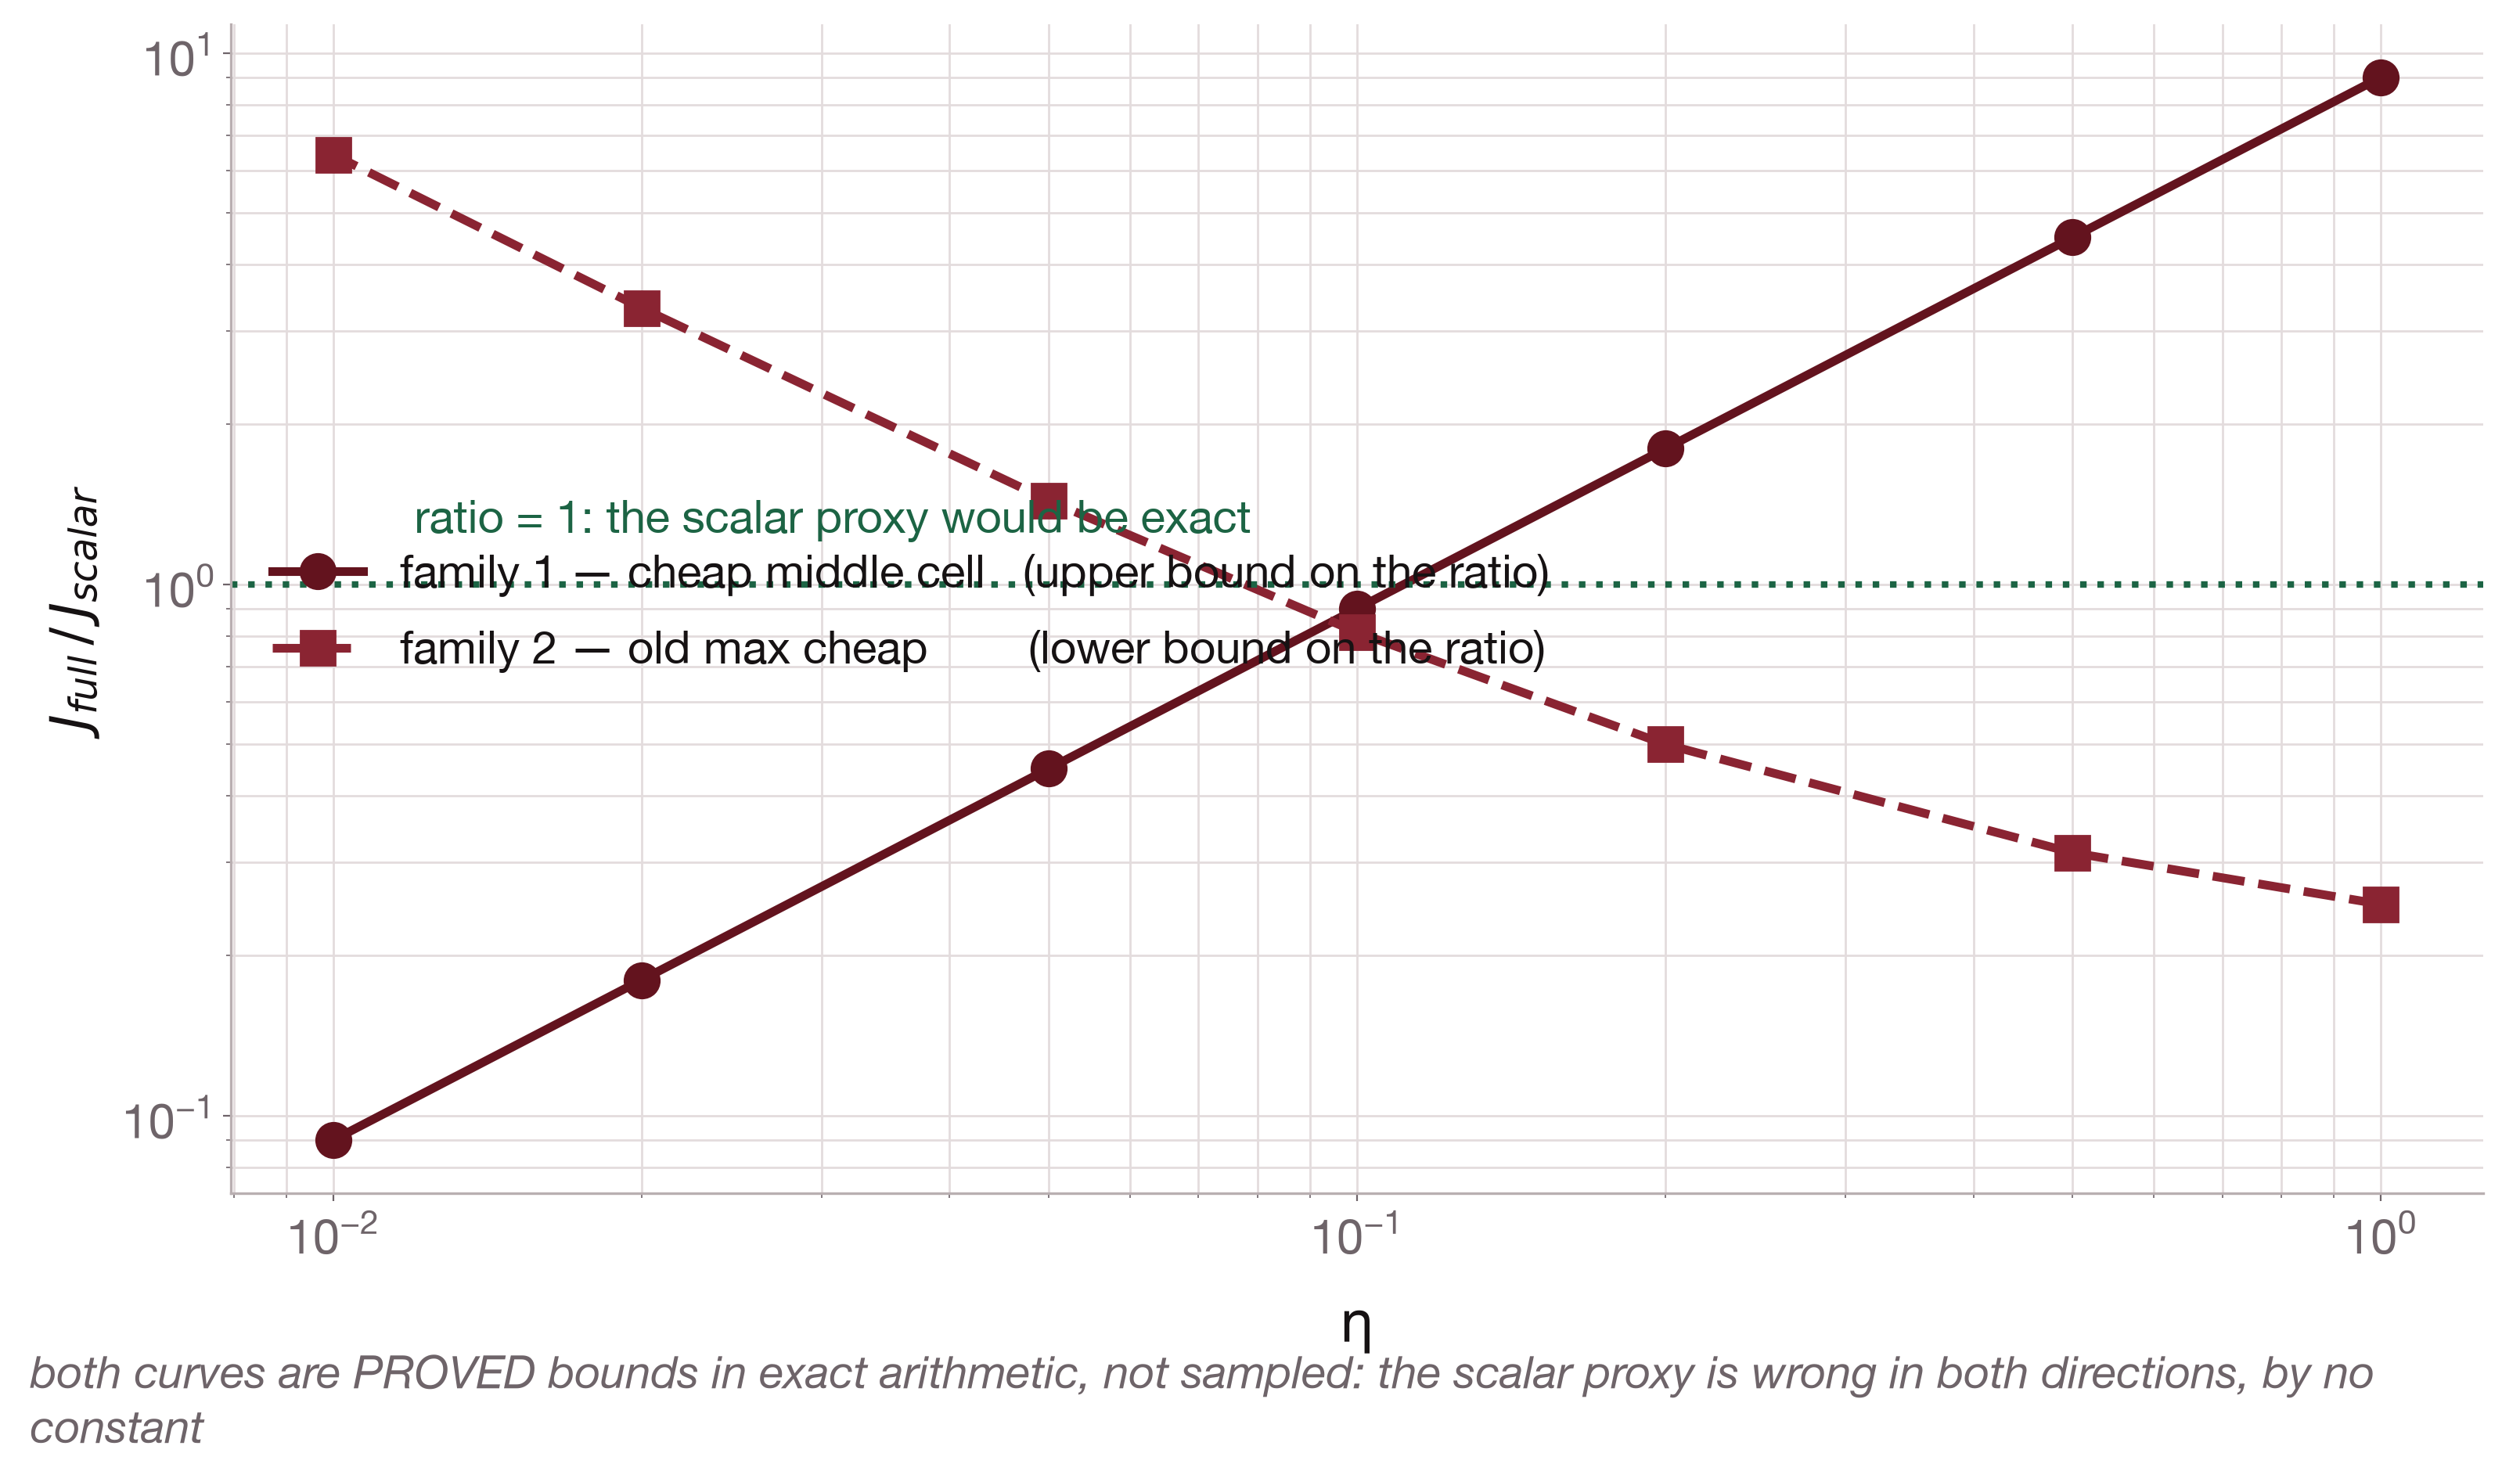
\includegraphics[width=\columnwidth]{func_fig2_families.png}
\caption{The two families of Section~\ref{sec:families}. Family 1 forces the ratio below
$9\eta$ and family 2 above $(1+3\eta)/(16\eta)$. Both curves are \emph{proved} bounds in
exact arithmetic, not sampled points: the failure of the scalar proxy is a theorem, and
Corollary~\ref{cor:noconstant} follows immediately from the two envelopes crossing every
horizontal line.}
\label{fig:families}
\end{figure}

\begin{table}[htbp]
\caption{The two families evaluated along the $\eta$ grid. Family 1's column is the proved
upper envelope $9\eta$ on $J_{\mathrm{full}}/J_{\mathrm{scalar}}$; family 2's is the proved
lower envelope $(1+3\eta)/(16\eta)$. They move in opposite directions, which is
Corollary~\ref{cor:noconstant}.}
\label{tab:families}
\centering
\footnotesize
\begin{tabular}{@{}rrr@{}}
\toprule
$\eta$ & Family 1 ratio $\le$ & Family 2 ratio $\ge$ \\
\midrule
$1.00$ & $9.0000$ & $0.2500$ \\
$0.50$ & $4.5000$ & $0.3125$ \\
$0.20$ & $1.8000$ & $0.5000$ \\
$0.10$ & $0.9000$ & $0.8125$ \\
$0.05$ & $0.4500$ & $1.4375$ \\
$0.02$ & $0.1800$ & $3.3125$ \\
$0.01$ & $0.0900$ & $6.4375$ \\
\bottomrule
\end{tabular}
\end{table}

\section{A worked certification}
\label{sec:worked}

The procedure of Section~\ref{sec:procedure} run on family~1 shows how the pieces fit, and
it is short enough to give in full.

The instance has $T=\{i\}$, one challenger $j$, three actions each. Step~1 enumerates the
ordered pairs $(a,b)$ of $j$: six of them. Consider the pair $(3,1)$, i.e.\ the region in
which $j$'s range is attained by its third cell above its first.

\emph{Step 2, shrink.} We may leave $i$ where it is, since inverting the capacities here is
cheaper through $j$; formally $S_{i}(z)=0$ for every $z\ge C_{i}(\mu)=1$.

\emph{Step 2, expand.} By \eqref{eq:expand} with $a=3$, $b=1$, $\theta_{j3}-\theta_{j1}
=\tfrac14$, precisions $\alpha_{j3}=\eta$ and $\alpha_{j1}=1$,
\begin{equation}
E_{j}(1)\;=\;\frac{\bigl[1-\tfrac14\bigr]_{+}^{2}}
                  {2\bigl(\tfrac{1}{\eta}+\tfrac{1}{1}\bigr)}
      \;=\;\frac{9/16}{2\,\frac{1+\eta}{\eta}}
      \;=\;\frac{9\eta}{32(1+\eta)} .
\end{equation}
Taking $\eta\to0$ this is $\tfrac{9\eta}{32}(1+O(\eta))$, matching the explicit
alternative used in the proof of Theorem~\ref{thm:family1}, which moves the single cell and
pays $\tfrac12\eta(\tfrac34)^{2}=\tfrac{9\eta}{32}$. The two agree because the explicit
alternative holds $j$'s first cell fixed while \eqref{eq:expand} allows it to move, and at
precision $1$ moving it is not worthwhile.

\emph{Step 5, minimise.} The remaining five pairs give values that do not fall with $\eta$,
because they route through cells of precision $1$. The minimum is therefore the pair
$(3,1)$ value, and $J_{\mathrm{full}}\le\tfrac{9\eta}{32}$.

\emph{What the proxy did instead.} Equation \eqref{eq:scalar} read $j$'s extrema off $\mu$
and found cells $2$ and $1$, both at precision $1$. It never formed the pair $(3,1)$, so the
region containing the cheapest alternative was never examined. The harmonic sum it computed
was $4$---the correct harmonic sum for the pair it did examine---and its answer,
$\tfrac{1}{32}$, is the correct value of the wrong problem.

This is worth stating in that form. The proxy is not an approximation with an error term; it
is an exact computation on a region that need not contain the minimiser.

\section{Setup cost and its crossing}
\label{sec:setup}

A design that switches support pays a setup cost, and comparing two supports requires
knowing where their budgets cross.

\begin{theorem}[Crossing budget]
\label{thm:crossing}
With per-support rates $\Gamma_{1}\neq\Gamma_{2}$, support sizes $|S_{1}|,|S_{2}|$ and setup
price $\kappa$,
\begin{equation}
B_{*}\;=\;\kappa\,\frac{|S_{2}|\,\Gamma_{2}-|S_{1}|\,\Gamma_{1}}{\Gamma_{2}-\Gamma_{1}} .
\label{eq:crossing}
\end{equation}
\end{theorem}

\leanbox{\lean{crossing\_budget}, \lean{infeasible\_iff} in
\lean{LeanFunctionalDesignDualityV1} and
\lean{LeanFunctionalRangeDesignCertificateV1}}

\begin{theorem}[Undetermined sign]
\label{thm:undecided}
If $\Gamma_{1}$ and $\Gamma_{2}$ are known only within brackets that overlap, both orders
$\Gamma_{1}<\Gamma_{2}$ and $\Gamma_{2}<\Gamma_{1}$ remain consistent with the data, so the
sign of the denominator in \eqref{eq:crossing} is undetermined and no crossing may be
reported.
\end{theorem}

\leanbox{\lean{crossing\_sign\_undetermined} in
\lean{LeanFunctionalRangeDesignCertificateV1}}

Theorem~\ref{thm:undecided} is a negative result stated deliberately. A procedure that
computes \eqref{eq:crossing} from bracketed inputs and reports whichever sign the midpoints
suggest will report a crossing that the data does not support. The honest output is
\textsc{undecided}.

\subsection{Deriving the crossing}

Equation \eqref{eq:crossing} is short enough to derive, and the derivation shows where each
quantity enters.

A design on support $S$ pays a setup cost $\kappa|S|$ once and then accrues value at rate
$\Gamma$ per unit of remaining budget. At total budget $B$ the value delivered is therefore
\begin{equation}
V_{S}(B)\;=\;\Gamma\,\bigl(B-\kappa|S|\bigr),
\label{eq:setupvalue}
\end{equation}
valid while $B\ge\kappa|S|$ and undefined below it---this is where
Proposition~\ref{prop:infeasible} applies, since a budget that does not cover the setup
admits no design on that support at all.

Two supports cross where $V_{S_{1}}(B)=V_{S_{2}}(B)$, i.e.\
$\Gamma_{1}(B-\kappa|S_{1}|)=\Gamma_{2}(B-\kappa|S_{2}|)$. Collecting $B$,
\begin{equation}
B\,(\Gamma_{1}-\Gamma_{2})\;=\;\kappa\bigl(\Gamma_{1}|S_{1}|-\Gamma_{2}|S_{2}|\bigr),
\end{equation}
and dividing by $\Gamma_{1}-\Gamma_{2}$, which is non-zero by hypothesis, gives
\eqref{eq:crossing}.

Three readings follow. Below $B_{*}$ the support with the smaller setup wins even though its
rate is worse, because the fixed cost dominates. Above $B_{*}$ the higher rate wins. And the
crossing moves linearly in $\kappa$: doubling the setup price doubles the budget at which
the larger support becomes worthwhile, which is the practically useful form of the law.

\subsection{Why the undetermined case must be reported}

Theorem~\ref{thm:undecided} says that if $\Gamma_{1}$ and $\Gamma_{2}$ are known only within
overlapping brackets, no crossing may be reported. The derivation above shows why this is
not pedantry. The denominator of \eqref{eq:crossing} is $\Gamma_{2}-\Gamma_{1}$; if its sign
is unknown, so is the direction of the inequality that $B_{*}$ separates, and a procedure
that substitutes bracket midpoints will report not merely an imprecise crossing but a
crossing pointing the wrong way. The failure is qualitative, not quantitative.

This is the same discipline as Section~\ref{sec:infeasible}: three outcomes rather than one,
with the degenerate cases named rather than encoded as numbers. It costs an implementation
two extra branches and it removes a class of silent errors that no amount of numerical care
would catch.

\begin{theorem}[Break-even, without the folklore 4]
\label{thm:breakeven}
\begin{equation}
\min_{p}\Bigl[\frac{\sigma_{a}^{2}}{p}+\frac{\sigma_{b}^{2}}{1-p}\Bigr]
=(\sigma_{a}+\sigma_{b})^{2},
\end{equation}
so break-even occurs at $c_{c}\nu_{c}=(\sigma_{a}+\sigma_{b})^{2}$.
\end{theorem}

\leanbox{\lean{scalar\_split\_optimal}, \lean{breakeven\_iff}, \lean{breakeven\_not\_four}
in \lean{LeanFunctionalDesignDualityV1}}

The number $4$ that circulates as a break-even threshold is the value of
$(\sigma_{a}+\sigma_{b})^{2}$ at unit variances and nothing more. With several alternatives
the scalar design shares cells and the pairwise threshold does not transfer; the statement
\lean{breakeven\_not\_four} records exactly this.

\section{Results}
\label{sec:results}

\subsection{The two families separate without limit}

As $\eta\to0$ the first family drives $J_{\mathrm{full}}/J_{\mathrm{scalar}}$ to zero and the
second drives it to infinity (Table~\ref{tab:families}, Fig.~\ref{fig:families}). Both are
proved bounds in exact arithmetic, not sampled points, so the failure of the proxy is a
theorem rather than an observation.

\subsection{On the main panel, $\mathrm{C\_lucb}$ is the baseline to beat}

\begin{table}[htbp]
\caption{Confirmatory panel, $1000$ paired instances. A result on this panel under this
generator, not a domination theorem.}
\label{tab:panel}
\centering
\footnotesize
\begin{tabular}{@{}lrrr@{}}
\toprule
Policy & certified & fraction & median $N$ \\
\midrule
$\mathrm{C\_lucb}$    & $797$ & $0.797$ & $20{,}996$ \\
$\mathrm{C\_anytime}$ & $749$ & $0.749$ & $29{,}884$ \\
uniform               & $605$ & $0.605$ & $74{,}252$ \\
\bottomrule
\end{tabular}
\end{table}

Where both certify---$749$ instances---$\mathrm{C\_lucb}$ is strictly faster in $748$, ties
in $1$ and loses in $0$, with a further $48$ worlds it certifies alone and $0$ that
$\mathrm{C\_anytime}$ certifies alone. This is a result \emph{on this panel under this
generator} and not a domination theorem, and the paper does not upgrade it into one.

\begin{figure}[htbp]
\centering
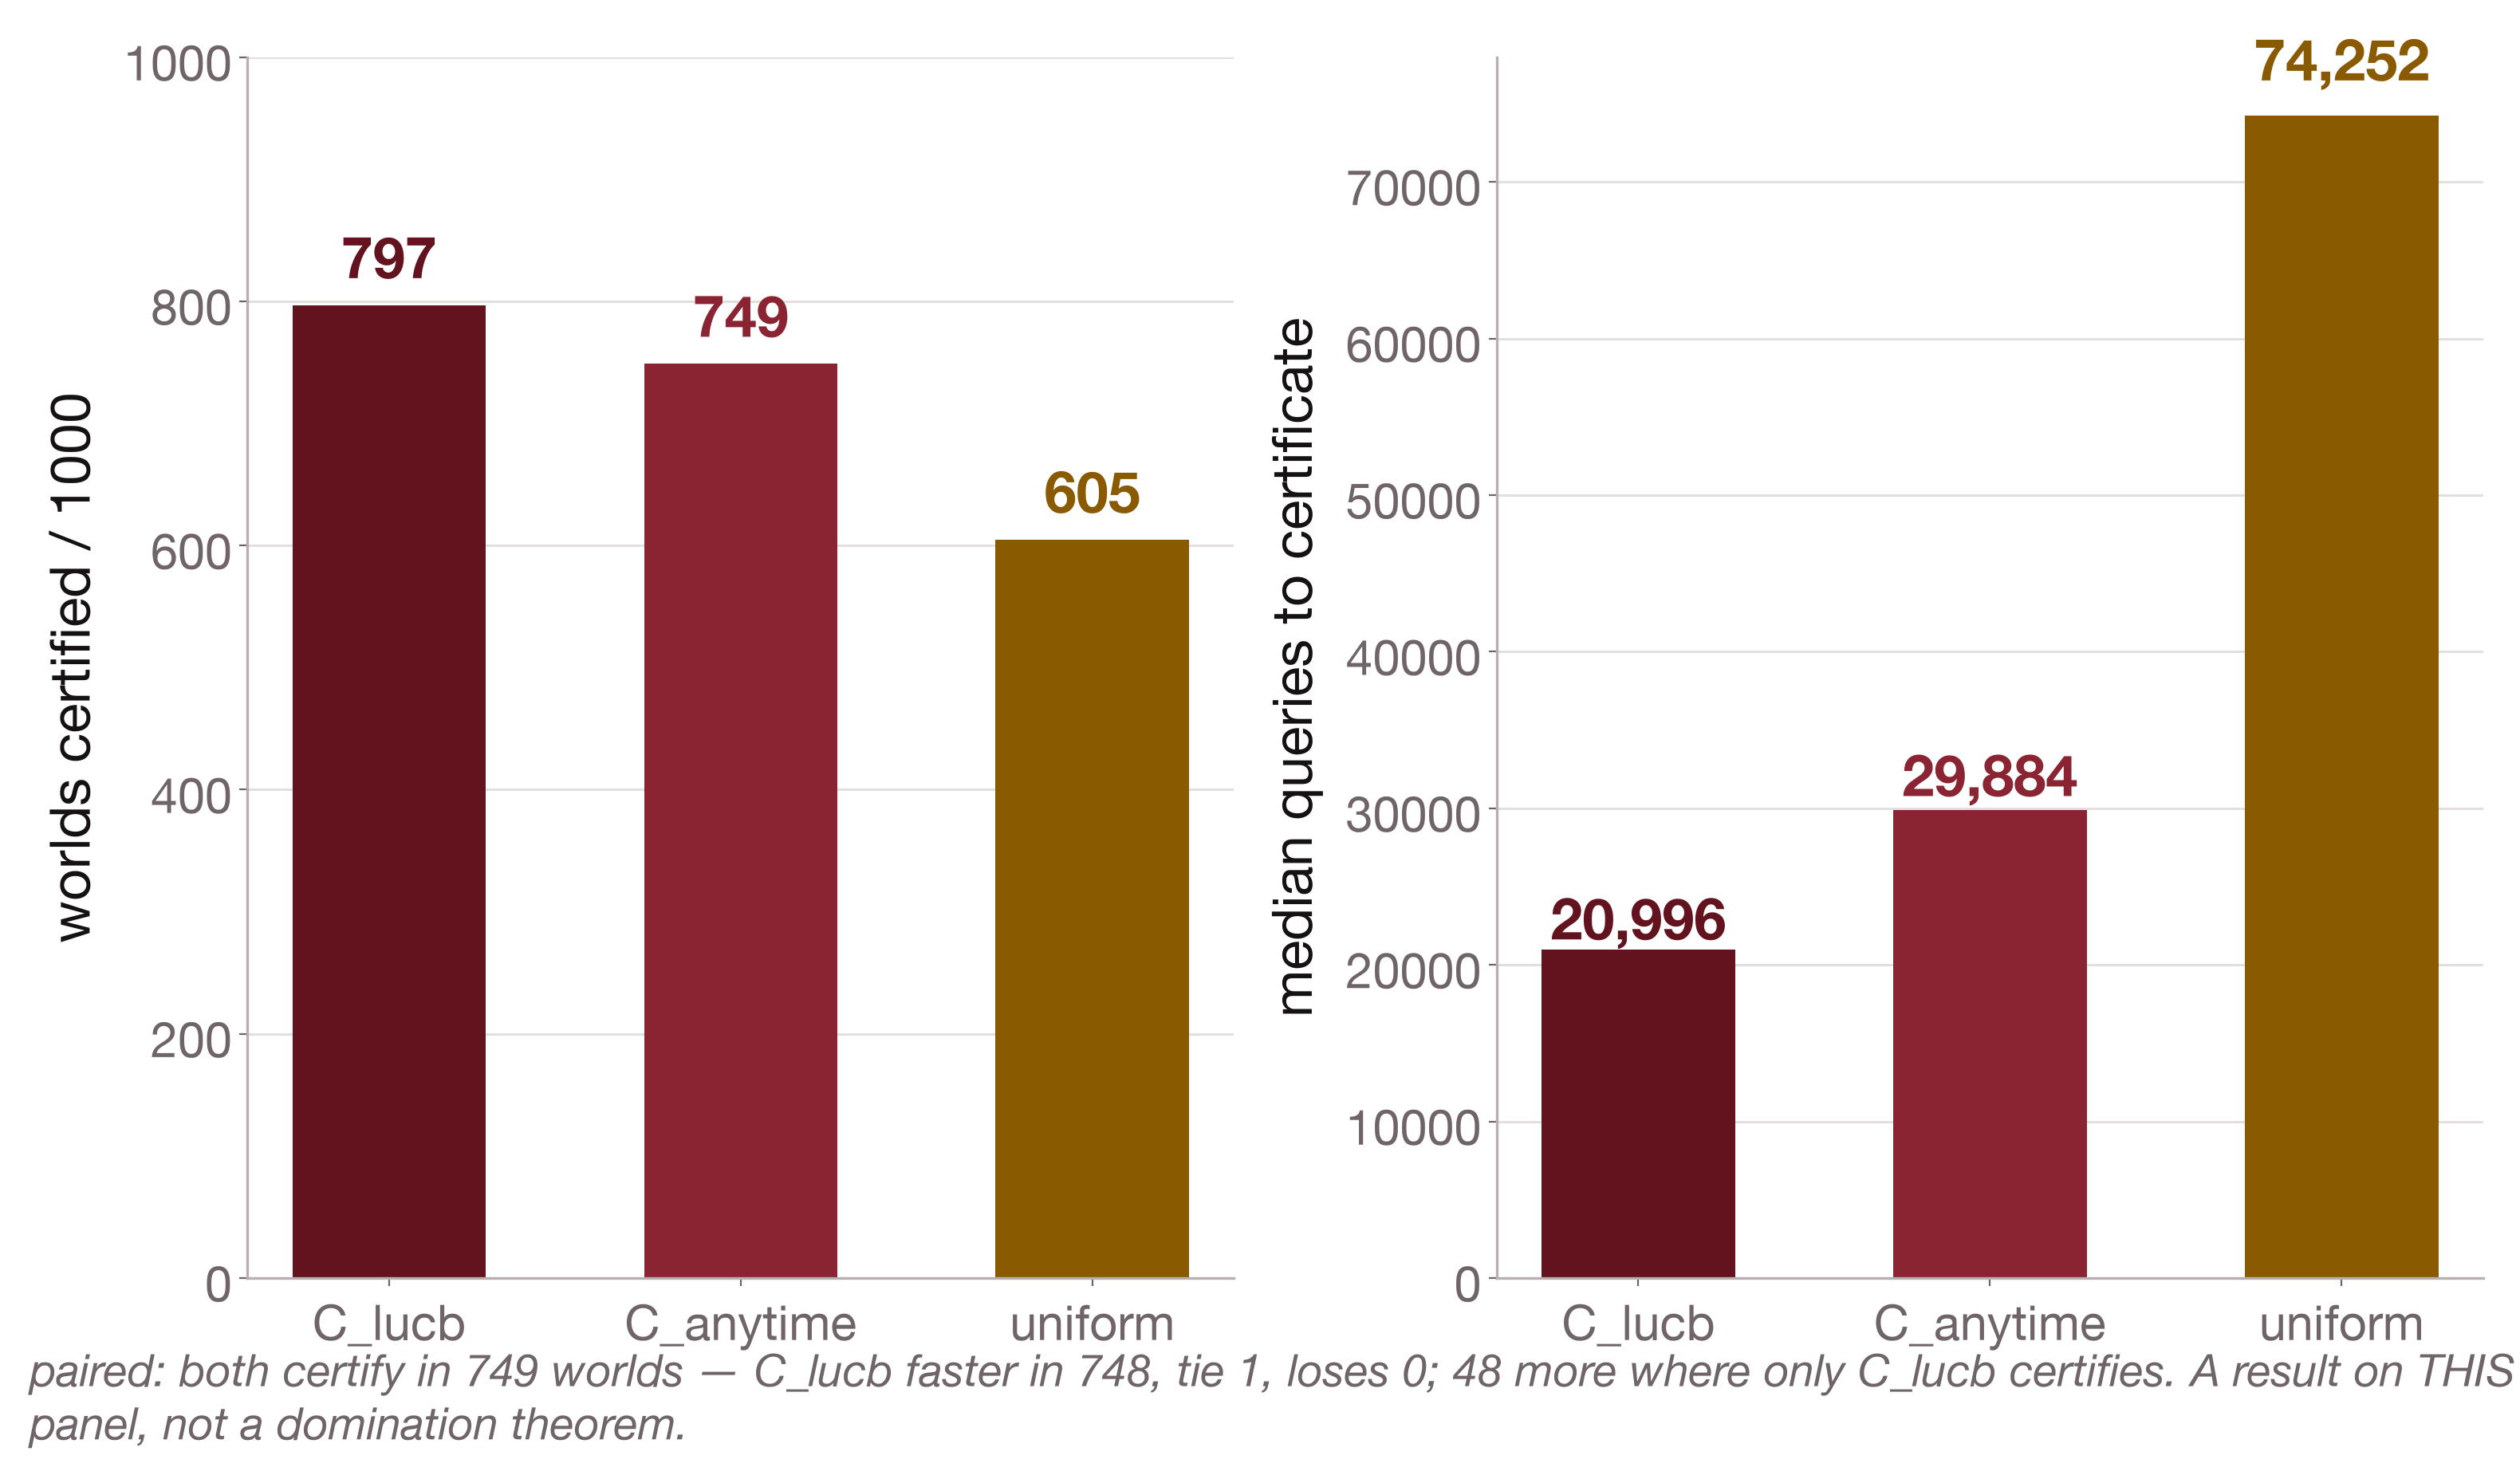
\includegraphics[width=\columnwidth]{func_fig1_panel.png}
\caption{The confirmatory panel, $1000$ paired instances at horizon $131{,}072$.
$\mathrm{C\_lucb}$ is the baseline any new allocator must beat, not a method this paper
defends: it certifies more worlds and certifies them faster than both comparators here.
Section~\ref{sec:discussion} notes that no allocator built on the oracle of
Sections~\ref{sec:union}--\ref{sec:kkt} has yet been compared against it.}
\label{fig:panel}
\end{figure}

\subsection{Reading the panel honestly}

Table~\ref{tab:panel} is a comparison among existing policies, and three things about it
should be stated rather than left to inference.

It is a panel result. The generator, the horizon and the instance distribution are fixed,
and a different generator could order the policies differently. Nothing here is a
domination theorem, and the paired analysis---$748$ strict wins, $1$ tie, $0$ losses out of
$749$ instances where both certify---is a property of these instances, not a proof that
$\mathrm{C\_lucb}$ is never slower.

It is not evidence for this paper's oracle. No allocator built on
Sections~\ref{sec:union}--\ref{sec:kkt} appears in the table. The panel is included because
it establishes which baseline a future allocator must beat, and the answer is
$\mathrm{C\_lucb}$ rather than uniform---a distinction that matters, since beating uniform
is easy and beating $\mathrm{C\_lucb}$ is the actual bar.

Censoring is substantial. $29.1\%$ of runs hit the horizon without certifying, so the
median $N$ figures are medians over certified runs and the certification fractions carry the
rest of the information. A policy that certified fewer worlds but faster on those it
certified would look good on median $N$ alone; reporting both columns is what prevents that
reading.

\subsection{Experiment scale}

The confirmatory panel is $10$ seeds $\times$ $1{,}000$ instances $\times$ $8$ policies
$=80{,}000$ policy runs at horizon $131{,}072$, drawing $5{,}042{,}978{,}194$ samples in
total, with $29.1\%$ of runs censored at the horizon. That is ten times the earlier panel,
and it ran as ten parallel processes for roughly six CPU-hours each. Every number reported
here comes from that run or from exact arithmetic; none is simulated for illustration.

\section{Infeasibility is not a small number}
\label{sec:infeasible}

One further discipline runs through the development and is easiest to state on its own.

A configuration in which no alternative inverts the capacities has \emph{no} finite value
for the infimum in \eqref{eq:J}: the feasible set is empty and the infimum is $+\infty$.
The temptation in an implementation is to return a large finite number, or worse a small
one, so that downstream arithmetic does not have to special-case it. Both are wrong, and the
second is dangerous: a small value reported for an infeasible configuration tells an
allocator that the answer is about to flip when in fact it cannot.

\begin{proposition}[Infeasibility is decidable and reported]
\label{prop:infeasible}
The emptiness of a pair region is characterised by an explicit condition on
$(\theta,\alpha)$, and the oracle returns \textsc{infeasible} rather than a numeric value in
that case.
\end{proposition}

\leanbox{\lean{infeasible\_iff} in \lean{LeanFunctionalDesignDualityV1}}

The same discipline produces Theorem~\ref{thm:undecided}. Where the inputs are bracketed
rather than known, the sign of the denominator in \eqref{eq:crossing} may be either, and the
output is \textsc{undecided}. Three outcomes---a value, \textsc{infeasible},
\textsc{undecided}---are therefore distinguished throughout, and the formal statements make
the distinction explicit rather than encoding it in a sentinel number.

\section{Formal verification}
\label{sec:verification}

Every theorem above is machine-checked in Lean~4, toolchain
\texttt{leanprover/lean4:v4.34.0-rc2} against mathlib revision \texttt{1f495c61}.

\subsection{Acceptance contract}

A module counts as accepted only when all six of the following hold: the compiler exits zero
with no errors; the source hash is unchanged \emph{across} the compile; the compiled
artifact is newer than its source; at least one \texttt{\#print axioms} directive is
present; the axiom set of every audited declaration lies within
$\{\textsf{propext},\textsf{Classical.choice},\textsf{Quot.sound}\}$; and no \texttt{sorry}
appears anywhere in the file.

\subsection{The crux statements as they are checked}

\begin{figure}[htbp]
\footnotesize
\hrule\vspace{4pt}
\begin{tabbing}
\quad\=\quad\=\kill
\lean{theorem scalar\_not\_upper\_to\_any\_constant} \\
\> \lean{(c : $\mathbb{R}$) (hc : 0 < c) :} \\
\> \lean{$\exists$ inst, Jfull inst < c * Jscalar inst} \\[6pt]
\lean{theorem scalar\_not\_lower\_to\_any\_constant} \\
\> \lean{(c : $\mathbb{R}$) (hc : 0 < c) :} \\
\> \lean{$\exists$ inst, c * Jscalar inst < Jfull inst} \\[6pt]
\lean{theorem kkt\_certificate} \\
\> \lean{(M : Matrix n n $\mathbb{R}$) (hsymm : M.IsSymm)} \\
\> \lean{(hpsd : $\forall$ v, 0 $\le$ v $\cdot$ (M.mulVec v))} \\
\> \lean{(hstat : M.mulVec (l - $\mu$) + A$^{\top}$.mulVec y = 0)} \\
\> \lean{(hdual : 0 $\le$ y) (hfeas : A.mulVec l $\le$ 0)} \\
\> \lean{(hcs : y $\cdot$ (A.mulVec l) = 0)} \\
\> \lean{($\lambda$' : n $\to$ $\mathbb{R}$) (hf : A.mulVec $\lambda$' $\le$ 0) :} \\
\> \lean{energy M $\mu$ l $\le$ energy M $\mu$ $\lambda$'}
\end{tabbing}
\vspace{-4pt}\hrule
\caption{The two-directional failure and the inverse-free certificate, as checked. The
first two statements are quantified over \emph{every} positive $c$, so they rule out any
constant correction rather than exhibiting one bad case;
Corollary~\ref{cor:noconstant} is their conjunction. In
\lean{kkt\_certificate} the hypothesis on $M$ is \lean{hpsd}, positive
\emph{semi}definiteness, and no invertibility or pseudoinverse appears in the statement or
in the proof.}
\label{fig:statements}
\end{figure}

The quantifier structure of the first two statements in Fig.~\ref{fig:statements} is the
whole content of C1. A theorem exhibiting one instance on which the proxy is bad would leave
open that a constant correction repairs it; these are stated with $c$ universally quantified
and the instance existential inside, so no constant survives. The instance produced is the
corresponding family with $\eta$ chosen from $c$.

\subsection{Evidence per step}

\begin{table}[htbp]
\caption{Evidence per step. All cited declarations are axiom-audited.}
\label{tab:inventory}
\centering
\footnotesize
\setlength{\tabcolsep}{3pt}
\begin{tabular}{@{}llr@{}}
\toprule
Step & Module & Aud. \\
\midrule
Union, Thm~\ref{thm:union}      & \lean{...RangeAlternativeUnionV1}  &  7 \\
Polyhedra, Prop~\ref{prop:convex} & \lean{...RangeAlternativeUnionV1} &  7 \\
Oracle, Thm~\ref{thm:oracle}    & \lean{...RangeEnergyOracleV1}      &  5 \\
Shrink/expand, Thms~\ref{thm:shrink}--\ref{thm:expand} & \lean{...ShrinkExpandV1} & 9 \\
Inner QP, Thm~\ref{thm:innerqp} & \lean{...RangeEnergyOracleV1}      &  5 \\
Certificate, Thm~\ref{thm:kkt}  & \lean{...RangeDesignCertificateV1} &  9 \\
Family 1, Thm~\ref{thm:family1} & \lean{...ScalarProxyFailsV1}       & 14 \\
Family 2, Thm~\ref{thm:family2} & \lean{...ScalarProxyFailsV1}       & 14 \\
Setup cost, Thms~\ref{thm:crossing}--\ref{thm:undecided} & \lean{...DesignDualityV1} & 21 \\
                                & \lean{...RangeDesignCertificateV1} &    \\
Break-even, Thm~\ref{thm:breakeven} & \lean{...DesignDualityV1}      & 12 \\
\bottomrule
\end{tabular}
\end{table}

All module names are prefixed \lean{LeanFunctional}, elided in the table for width.

\subsection{Scope of the formalisation}

The displayed results are the load-bearing chain, not the corpus. The Functional strand
contains $36$ Lean source files with $319$ theorem and lemma statements, of which $21$
modules carry an acceptance receipt covering $162$ declarations whose axiom set was printed
and checked. Across the programme of which this paper is one part: $427$ files, $3{,}115$
statements, $108$ accepted modules, $860$ audited declarations.

No module cited in this paper contains a \texttt{sorry}. Seven occurrences exist in the
wider repository, in audit scaffolding and in files named as conjectures; the overlap
between the cited set and the files containing them was computed and is empty.

\section{Discussion and scope}
\label{sec:discussion}

\subsection{What the families settle}

The two families settle a methodological question rather than a numerical one. Because the
proxy errs in both directions without a constant, no calibration of it can be safe: an
allocator that trusts it may either waste budget excluding an alternative that is already
cheap (family 1), or stop early against one that is far cheaper than it believes (family 2).
The correct object is the union of pair regions, and Theorem~\ref{thm:oracle} shows that
object is no harder to certify---it is a finite conjunction of convex problems.

\subsection{What is not established}

This section is longer than usual because the full oracle equality is \emph{not} assembled,
and saying so precisely is more useful than an optimistic summary.

\begin{enumerate}
\item \textbf{The decomposition step is not formalised.} That two relations occupy disjoint
blocks while every other relation stays at zero cost is a \emph{model} statement about the
observation structure, and it is what would be needed to assemble
Sections~\ref{sec:union}--\ref{sec:innerqp} into a full oracle equality. It is not proved
here, so the equality is not claimed. What is proved is each component of the chain
separately, plus the inequalities between them.

\item \textbf{Standing assumptions.} Free response table, known variance, positive
precision. Under realizability coupling the cost does not separate, and nothing here covers
that case.

\item \textbf{The certificate is sufficiency.} Theorem~\ref{thm:kkt} says a point with a
certificate is optimal. It does not say every optimal point has one.

\item \textbf{Only weak duality.} A duality gap is not excluded.

\item \textbf{No allocator has been built.} No allocator built on this oracle has yet been
compared against $\mathrm{C\_lucb}$, so Table~\ref{tab:panel} is a statement about existing
policies and not evidence for the oracle.
\end{enumerate}

\subsection{Why the scope section is long}

A paper whose main positive results are components of an oracle, rather than the oracle
itself, has an obligation to say exactly where the assembly stops. The obligation is
discharged above and the reason is worth naming.

The chain of Sections~\ref{sec:union}--\ref{sec:kkt} would become an equality
$J_{\mu}(x)=\min_{i,j}\inf_{z\ge0}[S_{i}(z)+E_{j}(z)]$ given one further statement: that in
the observation model the two relations $i$ and $j$ occupy disjoint blocks of the
information matrix while every other relation contributes zero cost to the alternative. That
statement is about the model, not about optimisation, and it is not proved here. Each
component of the chain is proved, and the inequalities between the three quantities in
\eqref{eq:order} are proved, so what is missing is precisely the separability step and
nothing else.

Stating this plainly costs the paper a headline. The alternative---presenting the chain as
though it closed---would make the paper's central discipline, that evidence classes are
never mixed, unavailable to it. The negative results of Section~\ref{sec:families} do not
depend on the assembly: they compare $J_{\mathrm{full}}$ against $J_{\mathrm{scalar}}$
directly, with $J_{\mathrm{full}}$ bounded above by an exhibited alternative in family~1 and
below by Lemma~\ref{lem:posparts} in family~2, neither of which uses separability.

\subsection{Why the certificate matters at the boundary}

Theorem~\ref{thm:kkt} is the result most likely to be reused, and the reason is
operational. An allocator that has learned something concentrates its budget, so its
information matrix loses rank; a certificate requiring $M^{-1}$ fails exactly when the
allocator is working well. Proving sufficiency from positive semidefiniteness removes that
failure mode at no cost---the proof is not longer than the invertible one, it simply avoids
the elimination step that introduces the inverse.

\subsection{What formalisation caught}

Three formulations were withdrawn under the prover.

The first version of the union identity froze the extrema at the truth: it quantified over
the pair $(a,b)$ attaining $\mu$'s extrema rather than $\lambda$'s. The forward direction of
Theorem~\ref{thm:union} then fails, because a maximiser of $\lambda_{j}$ need not be a
maximiser of $\mu_{j}$---which is precisely the phenomenon family~1 exploits. The
formalisation forced the quantifier to be over the alternative's extrema, and that change
is what made C2 a statement about the real target rather than about a surrogate.

The second was in the expand cost. An early \eqref{eq:expand} minimised over unordered
pairs, which double-counts: taking $\{a,b\}$ unordered forces the formula to consider the
case where the separation is already satisfied in the wrong direction, and the positive part
then hides a third cell that must move. The ordered form is what
\lean{range\_ge\_iff\_exists\_pair\_ge} states, and the difference is not cosmetic---the
unordered version overstates $E_{j}$ and would make the oracle report alternatives as more
expensive than they are.

The third was in the certificate. The first attempt followed the textbook route, eliminating
the primal variable with $M^{-1}$ and stating the dual. The hypothesis \lean{M.Nonsingular}
then propagated into every downstream statement, including the oracle, and would have made
the whole development inapplicable at sparse allocations. Restating the certificate as
sufficiency from \eqref{eq:kkt} removed the hypothesis entirely; the proof is no longer, and
Theorem~\ref{thm:kkt} now holds for every symmetric positive semidefinite $M$.

\subsection{What a practitioner loses by using the proxy}

The two families are extremal by construction, so it is fair to ask what happens on
ordinary instances. The honest answer is that the paper does not measure it, and the reason
is instructive: the size of the error depends on how far the cheapest alternative's
attaining cells are from the truth's, which is an instance property with no natural
distribution attached. A sweep over some generator would report a number that is a property
of the generator.

What the paper does establish is the shape of the risk, and it is asymmetric in
consequence. Family~1's failure---the proxy overstating---causes an allocator to keep
buying observations against an alternative that is already cheap to exclude, so the cost is
wasted budget and a late stop. Family~2's failure---the proxy understating---causes an
allocator to believe an alternative is nearly free and therefore already excluded, so the
cost is an \emph{early} stop and a wrong certificate. The second is a correctness failure
and the first is only an efficiency failure, which is a reason to care about the direction
of the error and not only its magnitude.

That asymmetry is also why Corollary~\ref{cor:noconstant} is stated in both directions
rather than in the one that is easier to prove. A one-sided result would leave open that
the proxy is conservative---always over-charging, hence safe if wasteful---and family~2
closes that route.

\subsection{Open problems}

Assembling the full oracle equality is the first and most important, and it requires the
separability statement named above rather than more optimisation. Building an allocator on
the exact oracle and comparing it against $\mathrm{C\_lucb}$ on the same panel is the
second; the present paper establishes that the exact oracle is computable and that the proxy
is unusable, but not that the exact oracle pays for itself. Whether strong duality holds for
the pair-region programme is the third. Finally, the families are two-relation and
three-action; whether the failure ratios can be driven to their limits with fewer actions,
or must worsen with more relations, is not known.

\section{Conclusion}

When the extrema can move, the scalar pair-flip proxy is a bound in neither direction, and
no constant repairs it. The true alternative set is a finite union of convex pair regions on
the real range target; its energy oracle is a finite conjunction of convex problems; the
inner problem has a closed form; and its optimality certificate needs no matrix inverse, so
a singular information matrix costs nothing extra. What remains is the decomposition step
that would turn these components into a single equality, and an allocator built on them.

For a practitioner the guidance is concrete. If relations are ranked by a mean, the
pair-flip value is exact and nothing here applies. If they are ranked by a range, or by any
statistic whose attaining cells can move, do not compute the value at the current extrema:
enumerate the ordered pairs, evaluate the shrink and expand costs on each, and take the
minimum. The enumeration is polynomial, each piece is a closed form, and the certificate
that the answer is right survives the singular information matrices that a concentrated
allocation produces.

\section*{Acknowledgment}

The formal development uses the Lean~4 theorem prover and the mathlib library.

\begin{thebibliography}{00}

\bibitem{jourdan2023} M. Jourdan, R. Degenne, and E. Kaufmann, ``Dealing with unknown
variances in best-arm identification,'' in \emph{Proc. 36th Annu. Conf. Learning Theory
(COLT)}, 2023.

\bibitem{garivier2016} A. Garivier and E. Kaufmann, ``Optimal best arm identification with
fixed confidence,'' in \emph{Proc. 29th Annu. Conf. Learning Theory (COLT)}, 2016.

\bibitem{boyd2004} S. Boyd and L. Vandenberghe, \emph{Convex Optimization}. Cambridge,
U.K.: Cambridge Univ. Press, 2004.

\bibitem{mathlib2020} The mathlib Community, ``The Lean mathematical library,'' in
\emph{Proc. 9th ACM SIGPLAN Int. Conf. Certified Programs and Proofs (CPP)}, 2020,
pp.~367--381.

\bibitem{demoura2021} L. de Moura and S. Ullrich, ``The Lean 4 theorem prover and
programming language,'' in \emph{Proc. 28th Int. Conf. Automated Deduction (CADE)}, 2021,
pp.~625--635.

\bibitem{kaufmann2016} E. Kaufmann, O. Capp\'e, and A. Garivier, ``On the complexity of
best-arm identification in multi-armed bandit models,'' \emph{J. Mach. Learn. Res.},
vol.~17, pp.~1--42, 2016.

\bibitem{rockafellar1970} R. T. Rockafellar, \emph{Convex Analysis}. Princeton, NJ:
Princeton Univ. Press, 1970.

\end{thebibliography}

\end{document}
